\documentclass{natourDoc}
\usepackage{lipsum}
\usepackage{tabularx}
\usepackage[table]{xcolor}
\usepackage{multirow}
\usepackage{float} 
\usepackage{svg}
\usepackage{amsmath}
\usepackage{pdfpages}
\usepackage{placeins}
\usepackage{hyperref}
\hypersetup{
    colorlinks=true,
    linkcolor=black,
    filecolor=magenta,
    urlcolor=blue,
    }

%\newcolumntype{a}{>{\columncolor{PineGreen!70}}l}

\def\arraystretch{1.5}

\title{Documentazione IngSW} %Titolo

\begin{document}

%----------- Informazioni --------------------

\titolo{Specifica, progettazione, implementazione e validazione del Sistema Informativo\\ \textit{NaTour21}} %Titolo.pdf
\sottotitolo{Dipartimento di Ingegneria Elettrica \\ e delle Tecnologie dell'Informazione} %Nome progetto

\professors{Sergio \textsc{Di Martino} \\
Francesco \textsc{Cutugno}} %Nome docenti

\students{Bianca Giada \textsc{Chehade} N86003209 \\
Mario \textsc{Liguori} N86003258\\ 
Mattia \textsc{Rossi} N86003211} %Nome studenti

%----------- Inizializzazione -----------------

\marginscreate %Crea margini
\cover %Crea cover
\toc %Crea Table of Contents

%------------ Corpo del documento ----------------

% \section{Première section} 

% \lipsum[3-4]%LOREMIPSUM

% \subsection{Subsection}

% \lipsum[3-4] %LOREMIPSUM

% \section{Deuxième section}

% \lipsum[3-5] %LOREMIPSUM

%------------- Comandi utili ----------------

% \section{Quelques commandes}

% Voici quelques commandes utiles :

%------ Per inserire immagini centrate ------

%\insertfigure{logos/logo.png}{3cm}{Légende de la figure}{Label de la figure}
% Le premier argument est le chemin pour la photo
% Le deuxième est la hauteur de la photo
% Le troisième la légende
% Le quatrième le label
%Ici, je cite l'image \ref{fig: Label de la figure}


%------- Per inserire un equazione --------------

% \begin{equation} \label{eq: exemple}
	% \rho + \Delta = 42
	% \end{equation}
	
	% L'équation \ref{eq: exemple} est cité ici. 
	
	% ------- Per inserire simboli/variabili ----------------------
	
	% Pour écrire des variables dans le texte, il suffit de mettre le symbole \$ entre le texte souhaité comme : constante $\rho$. 
	
	\section{Descrizione del progetto}
	NaTour21 è un sistema complesso e distribuito finalizzato ad offrire un moderno social network multipiattaforma per appassionati di escursioni.\\
	
	Il sistema consiste in:
	\begin{itemize}
		\item un Back-End sicuro, performante e scalabile;
		\item un client mobile attraverso cui gli
		utenti possono fruire delle funzionalità del sistema in modo intuitivo, rapido e piacevole;
		\item un client mobile attraverso cui gli amministratori possono gestire i contenuti inseriti in piattaforma.\\
	\end{itemize}
	
	NaTour21 ha lo scopo di creare una community sicura e affidabile dove condividere la propria passione per l'escursionismo.\\
	
	In questo scenario, l'utente si configura come protagonista: oltre alla possibilità di inserire itinerari (dettagliati da informazioni), compilation e post personali sulla piattaforma,
	è lasciato ampio spazio all'individualità personale.\\
	
	Tutto ciò si concretizza con la possibilità di interagire con gli altri utenti, in modo da poter avere un contatto più diretto con
	la realtà dell'escursionismo, e di lasciare valutazioni personali su qualunque itinerario si desideri.\\
	
	Il sistema valuta essenziale la sicurezza degli utenti: questi potranno segnalare informazioni inesatte o contenuti inappropriati al fine 
	di rendere la permanenza nella community piacevole per tutti.

	\subsection{Presentazione dell'idea progettuale}

	L'applicazione "NaTour21" nasce in seguito all'esigenza di uno spazio virtuale dove poter condividere la passione per l'escursionismo.\\
	Creare una community di escursionisti, esperti o meno, ha lo scopo di rendere le esperienze individuali degli utenti più sicure e informate, 
	oltre a promuovere la condivisione di contenuti personali.\\\\
	NaTour21 mette a disposizione degli utenti registrati diverse funzionalità.\\
	Il lato prettamente informativo consente di ricercare - nonchè inserire in piattaforma - diversi itinerari, e tutte le informazioni relative ad essi.
	Ciò comprende la possibilità di visualizzarli su mappa, e, per garantire un'accuratezza maggiore delle informazioni, di lasciare 
	un feedback personale per ciascuno di essi.\\\\
	Ci sono, però, ulteriori funzionalità che coinvolgono direttamente l'utente: tra queste la condivisione di post, la creazione di compilation personalizzate e 
	la visualizzazione di una homepage con post riguardanti diversi itinerari.\\
	Particolare attenzione è riservata alla sicurezza degli utenti, i quali possono segnalare contenuti inappropriati o informazioni inesatte.
	
	\subsection{Individuazione del target degli utenti}
	NaTour21 si configura come community in cui chiunque può intraprendere la passione per l'escursionismo e condividerla.\\\\
	Ciononostante, è stato possibile individuare un target di utenti ben definito grazie ai dati 
	statistici\footnote{Fonte: \href{http://dati.istat.it/Index.aspx?DataSetCode=DCCV_ESC_CAPI}{sito ufficiale Istat}.} raccolti 
	nell'anno 2020 dall'ISTAT, Istituto Nazionale di Statistica.\\\\
	In seguito all'analisi delle informazioni statistiche sull'escursionismo italiano è stato individuato come target utenti la popolazione, caratterizzata da un 
	numero di circa pari entità di uomini e di donne, nella fascia di età \texttt{35-64}. La maggior parte della 
	platea considerata risulta essere appartenente alla condizione lavorativa di \textit{dirigente, quadro o impiegato}.\\\\
	\begin{figure}[!htbp]
		\centering
		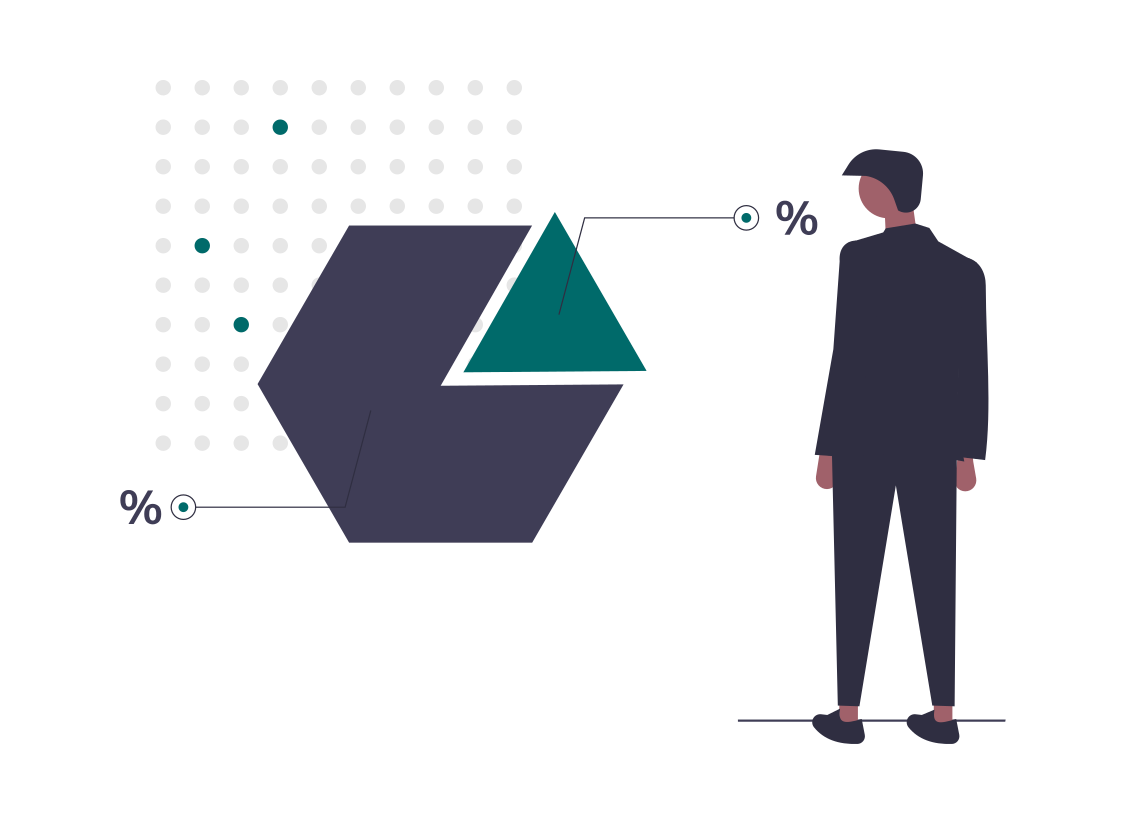
\includegraphics[width=12cm, page=1]{./logos/undraw_statistic_chart_38b6.png}
	\end{figure}
	\FloatBarrier
	L'Istat ha inoltre conteggiato nell'anno 2020 circa \texttt{41194} escursioni giornaliere,
	di cui il \texttt{42.7\%} situate temporalmente nel terzo trimestre dell'anno. Da questa informazione si deduce che il periodo
	preferito per attività escursionistiche sia quello dei mesi estivi.\\\\
	Il motivo prevalente per queste escursioni risulta essere stato \textit{piacere personale, svago e tempo libero}, con un numero
	di escursioni così orientate pari a \texttt{23223}: questo dato risulta particolarmente significativo, pari a un ordine
	di grandezza in più rispetto agli altri motivi registrati. È importante anche notare quanto il numero di escursioni in paesi 
	esteri sia di gran lunga minore rispetto a quelle nelle regioni italiane.\\\\
	Le regioni del Nord Italia sembrano essere state le preferite per visite giornaliere (la più visitata è stata il Veneto, con una media di
	\texttt{6200}), seguite immediatamente da quelle del centro-Sud. Il Molise, invece, non risulta aver raggiunto 
	la minima cifra considerata nella raccolta dati.\\

	\subsection{Definizione delle personas}

	\section{Documento dei Requisiti Software}
	\subsection{Requisiti funzionali}
	In questa sezione saranno esposti i requisiti \textit{funzionali} dell'applicazione NaTour21, cioè le funzionalità richieste dai commissionanti.
	
	\subsubsection{Autenticazione}
	\begin{table}[H]
		\centering
		\begin{tabular}{ |p{5cm}|p{10.3cm}| } 
			\hline
			\rowcolor{PineGreen!70}
			\textbf{Nome} & \textbf{Descrizione} \\
			\hline
			Registrazione & Il sistema deve consentire ad un utente di potersi registrare indicando e-mail e password, oppure utilizzando account di terze parti (Google o Facebook).\\ 
			\hline
		\end{tabular}
		\caption{RF.1}
		\label{table:1}
	\end{table}
	
	\begin{table}[H]
		\centering
		\begin{tabular}{ |p{5cm}|p{10.3cm}| } 
			\hline
			\rowcolor{PineGreen!70}
			\textbf{Nome} & \textbf{Descrizione} \\
			\hline
			Accesso & Il sistema deve consentire ad un utente di poter effettuare l'accesso alla piattaforma.\\ 
			\hline
		\end{tabular}
		\caption{RF.2}
		\label{table:2}
	\end{table}

	\begin{table}[H]
		\centering
		\begin{tabular}{ |p{5cm}|p{10.3cm}| } 
			\hline
			\rowcolor{PineGreen!70}
			\textbf{Nome} & \textbf{Descrizione} \\
			\hline
			Reimpostazione password & Il sistema deve consentire ad un utente registrato di poter cambiare la propria password se dimenticata o persa.\\ 
			\hline
		\end{tabular}
		\caption{RF.3}
		\label{table:3}
	\end{table}


	\subsubsection{Interazione con un itinerario}
	\begin{table}[H]
		\centering
		\begin{tabular}{ |p{5cm}|p{10.3cm}| }
			\hline
			\rowcolor{PineGreen!70}
			\textbf{Nome} & \textbf{Descrizione} \\
			\hline
			Visualizzazione itinerari & Il sistema deve consentire a un utente autenticato di visualizzare i
			dettagli degli itinerari pubblicati e i post ad essi associati. \\
			\hline
		\end{tabular}
		\caption{RF.4}
		\label{table:4}
	\end{table}

	\begin{table}[H]
		\centering
		\begin{tabular}{ |p{5cm}|p{10.3cm}| } 
			\hline
			\rowcolor{PineGreen!70}
			\textbf{Nome} & \textbf{Descrizione} \\
			\hline
			Inserimento itinerario &  Il sistema deve consentire a un utente autenticato di inserire nuovi itinerari (sentieri) in piattaforma. Un sentiero è
			caratterizzato da un nome, una durata, un livello di difficoltà, un punto di inizio, delle foto (max 5), una descrizione
			(opzionale), e un tracciato geografico (opzionale) che lo rappresenta su una mappa. Il tracciato
			geografico può essere inseribile manualmente (interagendo con una mappa interattiva) oppure
			tramite file in formato standard GPX.\\ 
			\hline
		\end{tabular}
		\caption{RF.4}
		\label{table:4}
	\end{table}
	
	\begin{table}[H]
		\centering
		\begin{tabular}{ |p{5cm}|p{10.3cm}| } 
			\hline
			\rowcolor{PineGreen!70}
			\textbf{Nome} & \textbf{Descrizione} \\
			\hline
			Ricerca itinerari &  Il sistema deve consentire a un utente autenticato di effettuare ricerche di itinerari tra quelli presenti in piattaforma, con possibilità di filtrare i risultati
			per area geografica, per livello di difficoltà, per durata, e per accessibilità ai disabili.\\ 
			\hline
		\end{tabular}
		\caption{RF.5}
		\label{table:5}
	\end{table}
	
	\begin{table}[H]
		\centering
		\begin{tabular}{ |p{5cm}|p{10.3cm}| } 
			\hline
			\rowcolor{PineGreen!70}
			\textbf{Nome} & \textbf{Descrizione} \\
			\hline
			Valutazione itinerario & Il sistema deve consentire a un utente autenticato di indicare un punteggio di difficoltà e/o un tempo
			di percorrenza diverso da quello indicato dall’utente che ha inserito il sentiero. In questo caso, il
			punteggio di difficoltà e il tempo di percorrenza per il sentiero saranno ri-calcolati come la media
			delle difficoltà/dei tempi indicati.\\ 
			\hline
		\end{tabular}
		\caption{RF.6}
		\label{table:6}
	\end{table}
	
	\begin{table}[H]
		\centering
		\begin{tabular}{ |p{5cm}|p{10.3cm}| }
			\hline
			\rowcolor{PineGreen!70}
			\textbf{Nome} & \textbf{Descrizione} \\
			\hline
			Salvataggio itinerario & Il sistema deve consentire a un utente autenticato di salvare gli itinerari
			nelle proprie compilation personalizzate. \\
			\hline
		\end{tabular}
		\caption{RF.7}
		\label{table:7}
	\end{table}

	\begin{table}[H]
		\centering
		\begin{tabular}{ |p{5cm}|p{10.3cm}| }
			\hline
			\rowcolor{PineGreen!70}
			\textbf{Nome} & \textbf{Descrizione} \\
			\hline
			Segnalazione itinerario & Il sistema deve consentire a un utente autenticato di segnalare degli itinerari
			le quali informazioni potrebbero non essere corrette e/o aggiornate. \\
			\hline
		\end{tabular}
		\caption{RF.8}
		\label{table:8}
	\end{table}

	\begin{table}[H]
		\centering
		\begin{tabular}{ |p{5cm}|p{10.3cm}| }
			\hline
			\rowcolor{PineGreen!70}
			\textbf{Nome} & \textbf{Descrizione} \\
			\hline
			Rimozione itinerario & Il sistema deve consentire a un utente autenticato di eliminare itinerari di cui
			è l'autore. \\
			\hline
		\end{tabular}
		\caption{RF.9}
		\label{table:9}
	\end{table}
	
	\subsubsection{Interazione con un post}
	\begin{table}[H]
		\centering
		\begin{tabular}{ |p{5cm}|p{10.3cm}| }
			\hline
			\rowcolor{PineGreen!70}
			\textbf{Nome} & \textbf{Descrizione} \\
			\hline
			Visualizzazione post & Il sistema deve consentire a un utente autenticato di visualizzare
			i dettagli di un post. \\
			\hline
		\end{tabular}
		\caption{RF.10}
		\label{table:10}
	\end{table}

	\begin{table}[H]
		\centering
		\begin{tabular}{ |p{5cm}|p{10.3cm}| } 
			\hline
			\rowcolor{PineGreen!70}
			\textbf{Nome} & \textbf{Descrizione} \\
			\hline
			Inserimento post &  Il sistema deve consentire a un utente autenticato di inserire un post, 
			caratterizzato da foto (max 5), una descrizione (opzionale) e un itinerario associato. \\
			\hline
		\end{tabular}
		\caption{RF.11}
		\label{table:11}
	\end{table}
	
	
	\begin{table}[H]
		\centering
		\begin{tabular}{ |p{5cm}|p{10.3cm}| }
			\hline
			\rowcolor{PineGreen!70}
			\textbf{Nome} & \textbf{Descrizione} \\
			\hline
			Segnalazione post & Il sistema deve consentire a un utente autenticato di segnalare post con fotografie
			inappropriate. \\
			\hline
		\end{tabular}
		\caption{RF.12}
		\label{table:12}
	\end{table}

	\begin{table}[H]
		\centering
		\begin{tabular}{ |p{5cm}|p{10.3cm}| }
			\hline
			\rowcolor{PineGreen!70}
			\textbf{Nome} & \textbf{Descrizione} \\
			\hline
			Rimozione post & Il sistema deve consentire a un utente autenticato di eliminare post di cui
			è l'autore. \\
			\hline
		\end{tabular}
		\caption{RF.13}
		\label{table:13}
	\end{table}
	
	\subsubsection{Gestione dati personali e conversazioni private}
	\begin{table}[H]
		\centering
		\begin{tabular}{ |p{5cm}|p{10.3cm}| } 
			\hline
			\rowcolor{PineGreen!70}
			\textbf{Nome} & \textbf{Descrizione} \\
			\hline
			Gestione profilo &  Il sistema deve consentire a un utente autenticato di gestire il suo profilo, 
			egli potrà visitare i contenuti inseriti ed eliminarli. Inoltre potrà cambiare la foto profilo. \\
			\hline
		\end{tabular}
		\caption{RF.14}
		\label{table:14}
	\end{table}

	\begin{table}[H]
		\centering
		\begin{tabular}{ |p{5cm}|p{10.3cm}| }
			\hline
			\rowcolor{PineGreen!70}
			\textbf{Nome} & \textbf{Descrizione} \\
			\hline
			Gestione conversazioni private & Il sistema deve permettere all'utente autenticato lo scambio di informazioni con altri utenti.
			È possibile avviare la conversazione a partire dai contenuti pubblicati. Inoltre è possibile ricercare un destinatario. \\
			\hline
		\end{tabular}
		\caption{RF.19}
		\label{table:19}
	\end{table}
	
	\subsubsection{Interazione con una compilation}
	\begin{table}[H]
		\centering
		\begin{tabular}{ |p{5cm}|p{10.3cm}| }
			\hline
			\rowcolor{PineGreen!70}
			\textbf{Nome} & \textbf{Descrizione} \\
			\hline
			Creazione compilation & Il sistema deve consentire a un utente autenticato di creare delle \textit{compilation personalizzate},
			caratterizzate da un titolo e da una descrizione. \\
			\hline
		\end{tabular}
		\caption{RF.16}
		\label{table:16}
	\end{table}

	\begin{table}[H]
		\centering
		\begin{tabular}{ |p{5cm}|p{10.3cm}| }
			\hline
			\rowcolor{PineGreen!70}
			\textbf{Nome} & \textbf{Descrizione} \\
			\hline
			Rimozione compilation & Il sistema deve consentire a un utente autenticato di eliminare le proprie
			compilation personalizzate \\
			\hline
		\end{tabular}
		\caption{RF.17}
		\label{table:17}
	\end{table}

	\begin{table}[H]
		\centering
		\begin{tabular}{ |p{5cm}|p{10.3cm}| }
			\hline
			\rowcolor{PineGreen!70}
			\textbf{Nome} & \textbf{Descrizione} \\
			\hline
			Visualizzazione compilation & Il sistema deve consentire a un utente autenticato di visualizzare i dettagli
			delle proprie compilation.  \\
			\hline
		\end{tabular}
		\caption{RF.15}
		\label{table:15}
	\end{table}

	
	\begin{table}[H]
		\centering
		\begin{tabular}{ |p{5cm}|p{10.3cm}| }
			\hline
			\rowcolor{PineGreen!70}
			\textbf{Nome} & \textbf{Descrizione} \\
			\hline
			Rimozione itinerario da compilation & Il sistema deve consentire a un utente autenticato di eliminare gli itinerari
			che compongono le proprie compilation personalizzate \\
			\hline
		\end{tabular}
		\caption{RF.18}
		\label{table:18}
	\end{table}

	\subsubsection{Requisiti amministratore}
	\begin{table}[H]
		\centering
		\begin{tabular}{ |p{5cm}|p{10.3cm}| }
			\hline
			\rowcolor{PineGreen!70}
			\textbf{Nome} & \textbf{Descrizione} \\
			\hline
			Visualizzazione segnalazioni & Il sistema deve permettere all'utente autenticato con i privilegi di amministratore di visualizzare
			la lista di segnalazioni inviate.\\
			\hline
		\end{tabular}
		\caption{RF.20}
		\label{table:20}
	\end{table}

	\begin{table}[H]
		\centering
		\begin{tabular}{ |p{5cm}|p{10.3cm}| }
			\hline
			\rowcolor{PineGreen!70}
			\textbf{Nome} & \textbf{Descrizione} \\
			\hline
			Amministrazione itinerario & Il sistema deve permettere all'utente autenticato con i privilegi di amministratore di modificare o
			rimuovere un itinerario segnalato.\\
			\hline
		\end{tabular}
		\caption{RF.21}
		\label{table:21}
	\end{table}

	\subsection{Requisiti non funzionali}
	Questa sezione conterrà invece i requisiti \textit{non funzionali} dell'applicazione, ovvero tutti i vincoli sui servizi offerti dal sistema.

	\begin{table}[H]
		\centering
		\begin{tabular}{ |p{5cm}|p{10.3cm}| } 
			\hline
			\rowcolor{PineGreen!70}
			\textbf{Nome} & \textbf{Descrizione} \\
			\hline
			Back-End scalabile & Il sistema deve essere scalabile e performante rispetto ai cambiamenti del Back-End,
			in modo da garantire un'agile manutenibilità nel tempo. \\
			\hline
		\end{tabular}
		\caption{RNF1}
		\label{table:21}
	\end{table}
	
	\begin{table}[H]
		\centering
		\begin{tabular}{ |p{5cm}|p{10.3cm}| } 
			\hline
			\rowcolor{PineGreen!70}
			\textbf{Nome} & \textbf{Descrizione} \\
			\hline
			Sicurezza password & Il sistema non consente di inserire password che non contengano 
			almeno 6 caratteri, di cui un carattere maiuscolo e un numero.\\
			\hline
		\end{tabular}
		\caption{RNF2}
		\label{table:22}
	\end{table}


	\begin{table}[H]
		\centering
		\begin{tabular}{ |p{5cm}|p{10.3cm}| } 
			\hline
			\rowcolor{PineGreen!70}
			\textbf{Nome} & \textbf{Descrizione} \\
			\hline
			Singola valutazione per itinerario & Il sistema non consente di inserire più di una valutazione
			per itinerario. \\
			\hline
		\end{tabular}
		\caption{RNF3}
		\label{table:23}
	\end{table}

	\begin{table}[H]
		\centering
		\begin{tabular}{ |p{5cm}|p{10.3cm}| } 
			\hline
			\rowcolor{PineGreen!70}
			\textbf{Nome} & \textbf{Descrizione} \\
			\hline
			Segnalazione unica per un post & Il sistema non consente di inviare più di una segnalazione per un post. \\
			\hline
		\end{tabular}
		\caption{RNF4}
		\label{table:24}
	\end{table}

	\begin{table}[H]
		\centering
		\begin{tabular}{ |p{5cm}|p{10.3cm}| } 
			\hline
			\rowcolor{PineGreen!70}
			\textbf{Nome} & \textbf{Descrizione} \\
			\hline
			Numero massimo di foto & Il sistema non consente di inserire più di 5 foto per itinerario o post. \\
			\hline
		\end{tabular}
		\caption{RNF5}
		\label{table:25}
	\end{table}

	\newpage

	\subsection{Requisiti di dominio}
	Infine, questa sezione conterrà i requisiti \textit{di dominio} dell'applicazione, ovvero tutti i vincoli generali a cui l'applicativo
	deve attenersi. \\

	\begin{table}[H]
		\centering
		\begin{tabular}{ |p{5cm}|p{10.3cm}| }
			\hline
			\rowcolor{PineGreen!70}
			\textbf{Nome} & \textbf{Descrizione} \\
			\hline
			ISO/IEC 27018:2019 & Il sistema deve essere conforme allo standard ISO/IEC 27018:2019, 
			incentrato sulla protezione dei dati personali nel cloud. \\
			\hline
		\end{tabular}
		\caption{RD1}
		\label{table:26}
	\end{table}

	\begin{table}[H]
		\centering
		\begin{tabular}{ |p{5cm}|p{10.3cm}| }
			\hline
			\rowcolor{PineGreen!70}
			\textbf{Nome} & \textbf{Descrizione} \\
			\hline
			GDPR & Il sistema deve essere conforme al GDPR (Regolamento Generale sulla Protezione dei Dati), 
			incentrato sul trattamento dei dati personali e sulla privacy dell’utente.  \\
			\hline
		\end{tabular}
		\caption{RD2}
		\label{table:27}
	\end{table}

	\newpage

	\newpage
	\subsection{Modellazione dei Casi d'Uso}
	In questa sezione sarà riportato il diagramma Use Case per l'applicazione.\\
	Per garantire una maggiore leggibilità e data la molteplicità di funzioni garantite
	dal sistema, si è fatta la scelta di raggruppare le funzioni logicamente legate 
	tra loro in packages.

	\begin{figure}[!htbp]
		\centering
		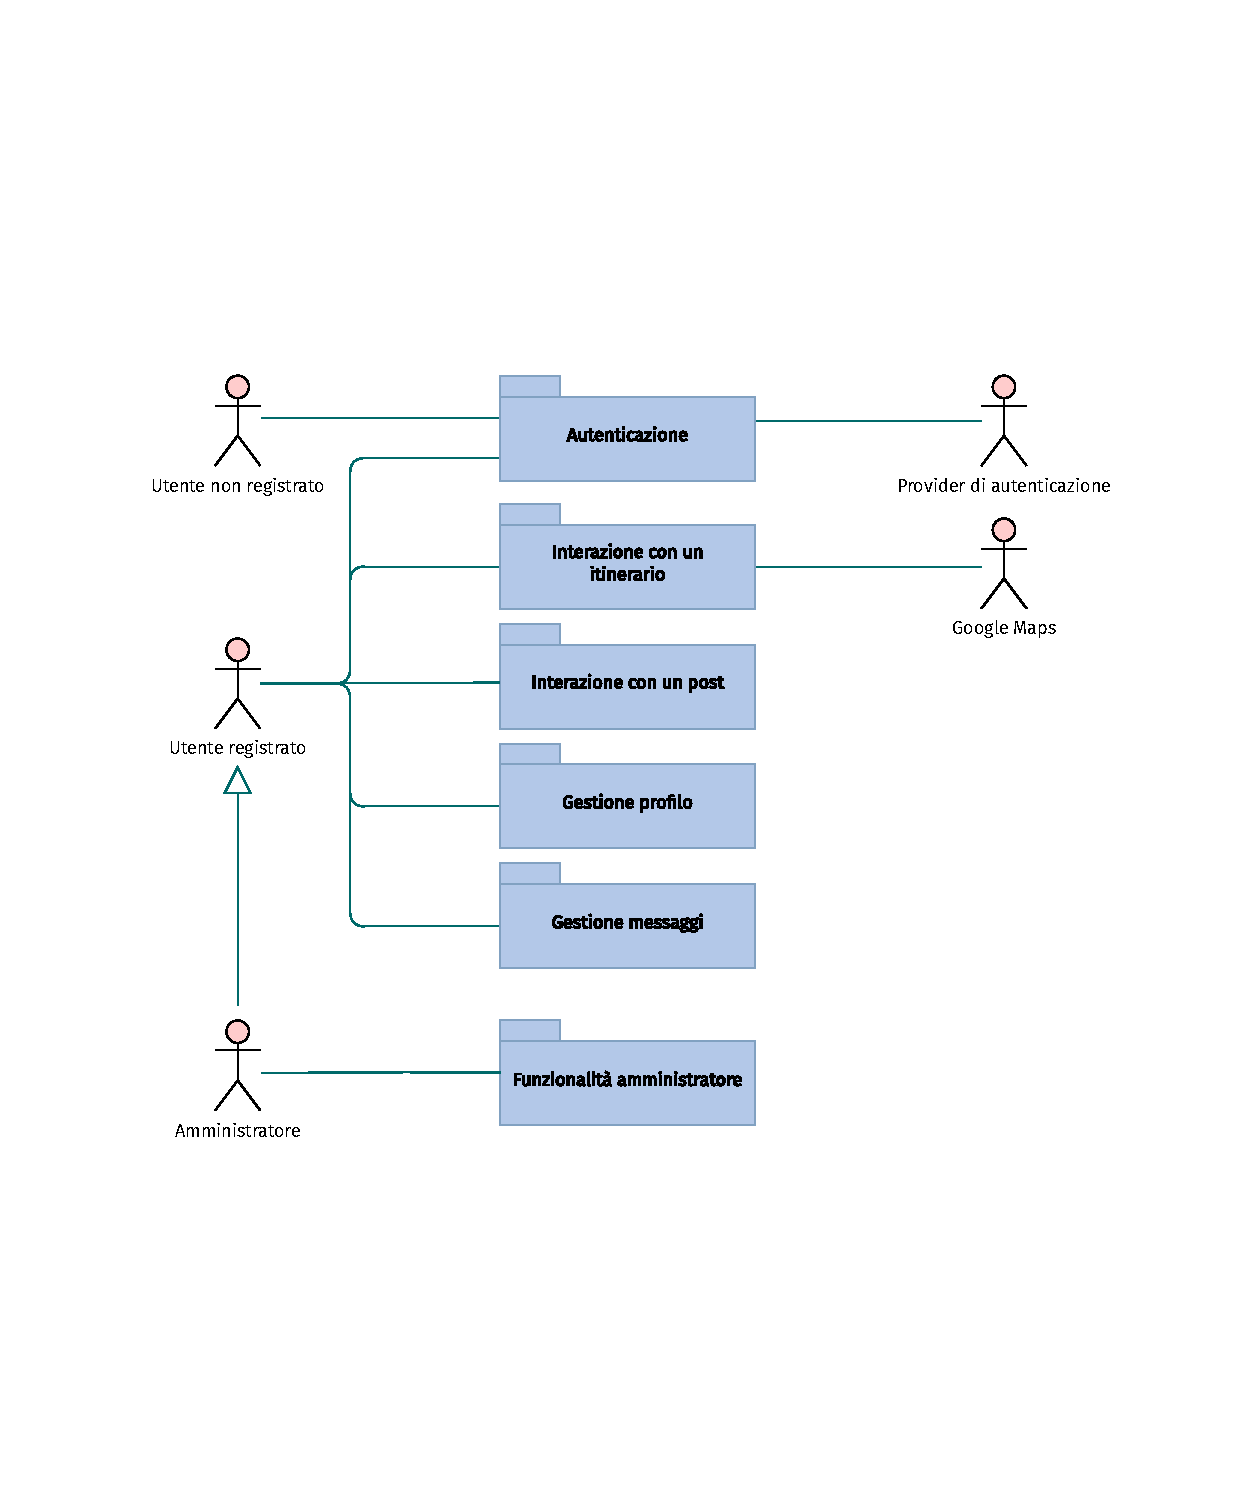
\includegraphics[width=\textwidth, page=1]{./diagrams/useCase.pdf}
		\caption{Use Case Diagram}
	\end{figure}
	\FloatBarrier

	\newpage
	\subsubsection{Interazione con un itinerario}
	\begin{figure}[!htbp]
		\centering
		\includegraphics[width=\textwidth, page=3]{./diagrams/useCase.pdf}
		\caption{Package 1 - Interazione con un Itinerario}
	\end{figure}
	\FloatBarrier

	\newpage
	\subsubsection{Interazione con un post}
	\begin{figure}[!htbp]
		\centering
		\includegraphics[width=\textwidth, page=4]{./diagrams/useCase.pdf}
		\caption{Package 2 - Interazione con un Post}
	\end{figure}
	\FloatBarrier

	\newpage
	\subsubsection{Gestione profilo}
	\begin{figure}[!htbp]
		\centering
		\includegraphics[width=\textwidth, page=5]{./diagrams/useCase.pdf}
		\caption{Package 3 - Gestione Profilo}
	\end{figure}
	\FloatBarrier

	\newpage
	\subsubsection{Gestione messaggi}
	\begin{figure}[!htbp]
		\centering
		\includegraphics[width=\textwidth, page=2]{./diagrams/useCase.pdf}
		\caption{Package 4 - Gestione messaggi}
	\end{figure}
	\FloatBarrier

	\newpage
	\subsection{Tabelle di Cockburn dei casi d'uso}
	Sono presentate in questa sezione le tabelle di Cockburn relative a due casi d'uso significativi dell'UCD.

	%%TODO
	
	\subsubsection{Inserisce un itinerario}
	
	%TODO
	
	\subsubsection{Segnala un itinerario}
	
	%TODO
	\newpage

	\subsection{Mock-Up dell'applicazione}
	Vengono ora mostrati i Mock-Up dei casi d'uso significativi dettagliati nella sottosezione precedente.\\
	Sarà specificato per ogni Mock-Up il tipo e la funzionalità di ogni componente.



	\subsection{Prototipazione funzionale via statechart dell'interfaccia grafica}

	\subsection{Classi, oggetti e relazioni di analisi}

	\subsection{Diagrammi di sequenza di analisi}

	\subsection{Diagrammi di attività}


	
	\section{Documento di Design del sistema}




\end{document}	